\chapter{Gauss's Law, Accelerated Frames, and Curvature}

\section{A Detour Through Dark Energy}

Before returning to Newtonian gravity, let us settle a question left over
from the preceding discussion. A positive cosmological constant contributes
a very weak repulsive effect whose magnitude grows with separation. For the
limited purpose at hand, a spring supplies a useful model. If its ordinary
restoring force is
\begin{equation}
  F_{\mathrm{spring}}=-kr,
\end{equation}
then the cosmological term may be represented schematically by
\begin{equation}
  F_{\mathrm{total}}=-(k-\lambda)r=-kr+\lambda r,
  \qquad 0<\lambda\ll k.
  \label{eq:l02-spring-lambda}
\end{equation}
The analogy is not meant to turn an atom into a literal spring. It isolates
the relevant point: adding a minute repulsive coefficient weakens a bound
system slightly. Its equilibrium dimensions shift by a negligible amount;
it is not torn apart. The same conclusion applies to laboratory systems,
the solar system, and ordinary galactic binding. The effect becomes
competitive only over cosmological distances.

\begin{figure}[tbp]
  \centering
  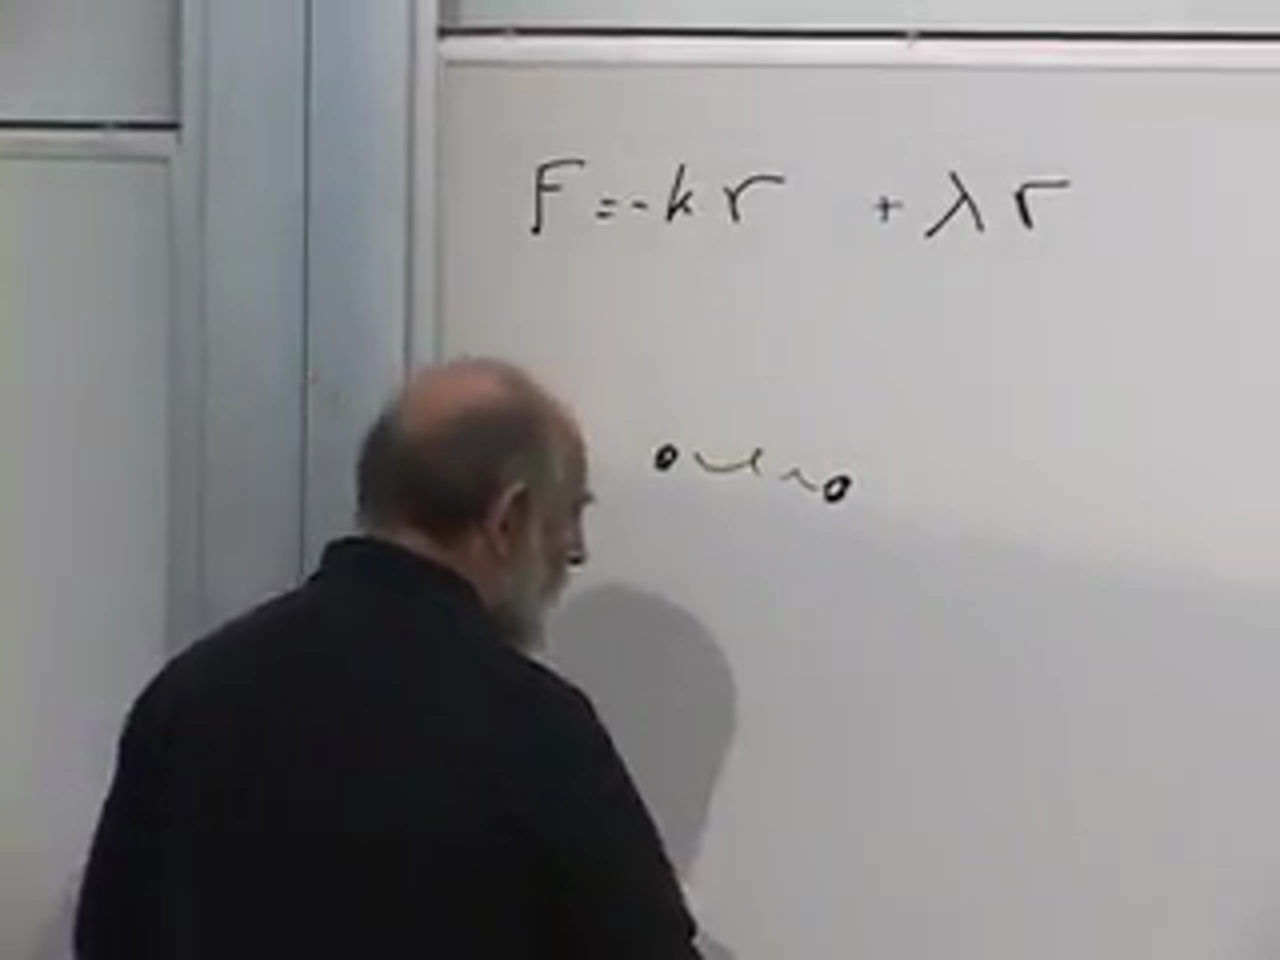
\includegraphics[width=0.76\textwidth]{lecture_02_figure_01.png}
  \caption{A spring supplies the opening model for a tiny repulsive
  cosmological contribution. The important comparison is between the strong
  restoring coefficient \(k\) and the exceedingly small coefficient
  \(\lambda\).}
  \lectureframe{00:05:00}
\end{figure}

This also separates an ordinary cosmological constant from the proposed
\emph{Big Rip}. A genuine constant does not grow in time. The rip scenario
instead assumes an effective repulsion that becomes progressively stronger,
first overcoming galactic binding, then stellar and planetary binding, and
eventually microscopic binding. That is a different hypothesis, and the
lecture treats a growing \(\lambda\) as physically implausible. A decreasing
dark-energy component is conceptually distinct and is not ruled out by the
same argument.

\begin{classroomqa}
\audiencequestion{Is \(\lambda\) a function of the mass, and would it still
exist if no particles were present?
\lecturetimestamp{00:08:47--00:09:16}}
\lecturerresponse{Here \(\lambda\) is a numerical constant, not a function
of a particular source mass. It specifies how particles would respond if
they were present. If there are no particles, there are simply no test
bodies on which to display that force.}
\end{classroomqa}

\begin{classroomqa}
\audiencequestion{Does the cosmological constant evolve with time?
\lecturetimestamp{00:09:16--00:09:49}}
\lecturerresponse{In the standard interpretation it is constant, which is
why the name is appropriate. More general forms of dark energy can vary.
The opening argument distinguishes a possible decrease from the strongly
disfavored increase required by the Big Rip.}
\end{classroomqa}

\begin{classroomqa}
\audiencequestion{How can dark energy be a large fraction of the cosmic
energy budget if its local effect is so small?
\lecturetimestamp{00:09:55--00:12:36}}
\lecturerresponse{Its density in a cubic meter is extraordinarily small.
What matters cosmologically is that this small density fills an enormous
volume smoothly. Accumulated over distances comparable with the observable
universe, its gravitational effect can dominate the expansion even though
it is irrelevant in the laboratory, the solar system, and most individual
astronomical systems. For the same reason it is not a practical reservoir
from which to extract a useful tankful of energy.}
\end{classroomqa}

\begin{classroomqa}
\audiencequestion{Is dark energy a relative energy, so that only differences
in it matter?
\lecturetimestamp{00:12:40--00:13:20}}
\lecturerresponse{The word \emph{relative} needs a more precise definition
before that question has a unique answer. The point retained here is that
dark energy gravitates: it acts as a smooth source in the large-scale
gravitational dynamics.}
\end{classroomqa}

\begin{classroomqa}
\audiencequestion{Is there a particle associated with dark energy?
\lecturetimestamp{00:13:25--00:14:01}}
\lecturerresponse{Not in the cosmological-constant picture used here. Dark
energy is not being described as a gas of particles. This is quite different
from dark matter, which is generally believed to consist of particles.}
\end{classroomqa}

That answers the questions which motivated the detour. We now need a little
more Newtonian gravity before we can move on to Einstein.

\section{Del, Gradients, and Divergences}

The necessary mathematics is mostly notation. Introduce the differential
operator
\begin{equation}
  \boldsymbol{\nabla}
  =
  \left(
    \frac{\partial}{\partial x},
    \frac{\partial}{\partial y},
    \frac{\partial}{\partial z}
  \right).
  \label{eq:l02-del}
\end{equation}
It resembles a vector because it has three components, but those components
are operations rather than numbers.

When \(\phi(x,y,z)\) is a scalar field, applying del produces its gradient,
a vector field:
\begin{equation}
  \boldsymbol{\nabla}\phi
  =
  \left(
    \frac{\partial\phi}{\partial x},
    \frac{\partial\phi}{\partial y},
    \frac{\partial\phi}{\partial z}
  \right).
  \label{eq:l02-gradient}
\end{equation}
For a vector field
\(\vec v=(v_x,v_y,v_z)\), taking the dot product with del gives the
divergence,
\begin{equation}
  \boldsymbol{\nabla}\cdot\vec v
  =
  \frac{\partial v_x}{\partial x}
  +\frac{\partial v_y}{\partial y}
  +\frac{\partial v_z}{\partial z}.
  \label{eq:l02-divergence}
\end{equation}
Just as the dot product of two ordinary vectors is a scalar, the divergence
of a vector field is a scalar field. A fleeting verbal reversal at the board
does not change this type: gradient maps scalar to vector; divergence maps
vector to scalar.

\begin{figure}[tbp]
  \centering
  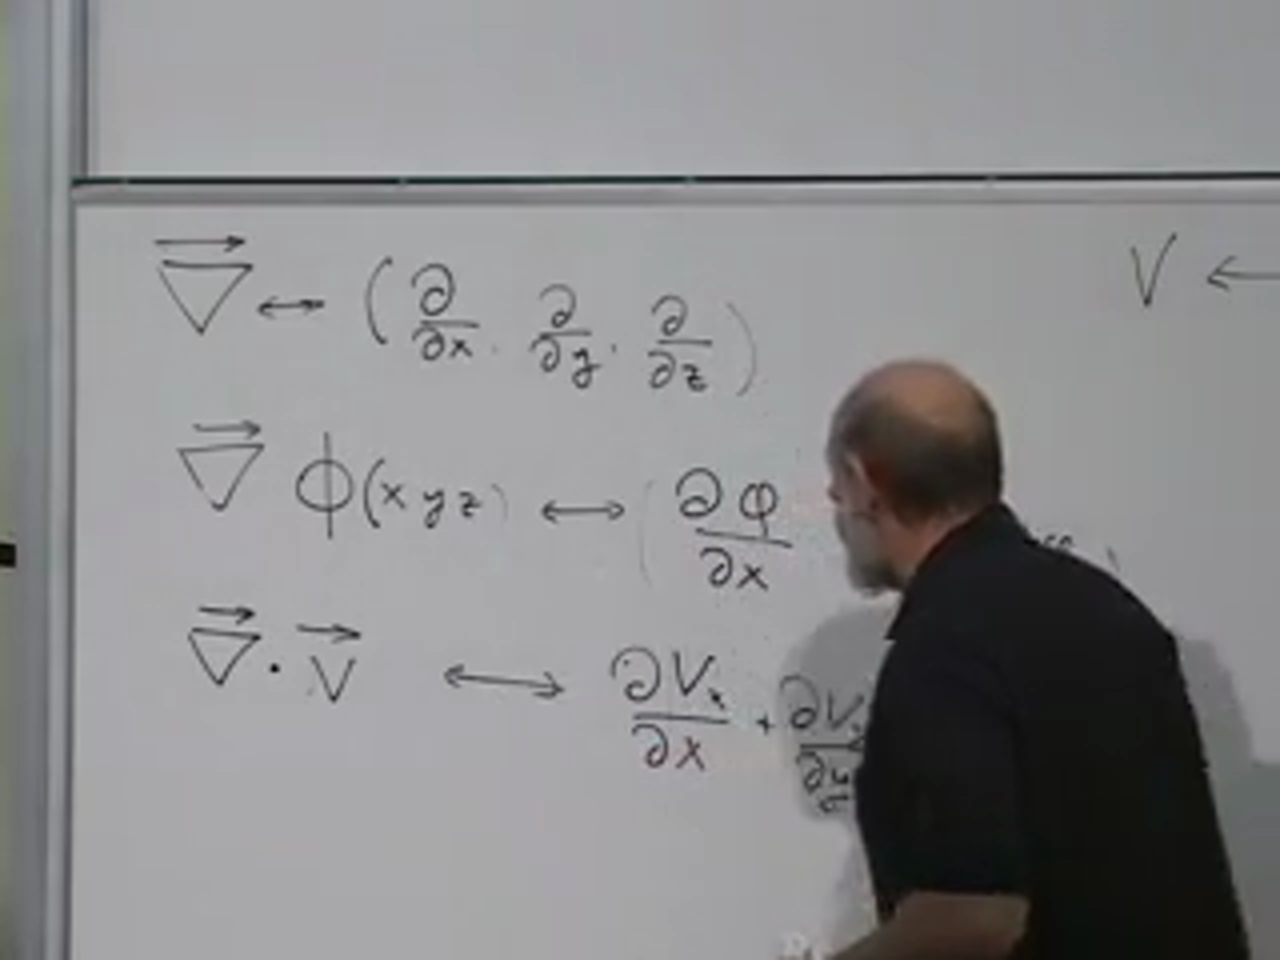
\includegraphics[width=0.82\textwidth]{lecture_02_figure_02.png}
  \caption{The del operator, the gradient of a scalar, and the divergence of
  a vector are assembled on one board. These operations will turn Newton's
  inverse-square law into a local field equation.}
  \lectureframe{00:19:30}
\end{figure}

A field is simply a quantity assigned at every point. If the assigned
quantity is a number, it is a scalar field; if it has magnitude and
direction, it is a vector field. The gravitational acceleration is our first
important vector field.

\section{The Gravitational Acceleration Field}

Imagine source masses \(m_i\) at positions \(\vec x_i\). To define the field
at \(\vec x\), place a test mass there, release it, and record its
acceleration. The test mass is chosen small enough that its own disturbance
of the sources can be neglected. Define
\begin{equation}
  \vec R_i=\vec x_i-\vec x,
  \qquad
  R_i=\lvert\vec R_i\rvert ,
  \qquad
  \widehat{\vec R}_i=\frac{\vec R_i}{R_i}.
  \label{eq:l02-source-vector}
\end{equation}
Thus \(\vec R_i\) points from the field point toward source \(i\). This
choice resolves the sign hesitation that occurs while the diagram is being
drawn: attraction is then along \(+\vec R_i\), and no extra minus sign is
needed.

The acceleration field is
\begin{equation}
  \boxed{
  \vec A(\vec x)
  =
  G\sum_i m_i\frac{\vec R_i}{R_i^3}
  =
  G\sum_i m_i\frac{\widehat{\vec R}_i}{R_i^2}.}
  \label{eq:l02-discrete-field}
\end{equation}
The unit-vector form displays the inverse-square magnitude. The
\(\vec R_i/R_i^3\) form packages magnitude and direction into a single
vector expression. Moving the test point changes every \(\vec R_i\), so
\(\vec A\) depends on position and is indeed a field.

\begin{figure}[tbp]
  \centering
  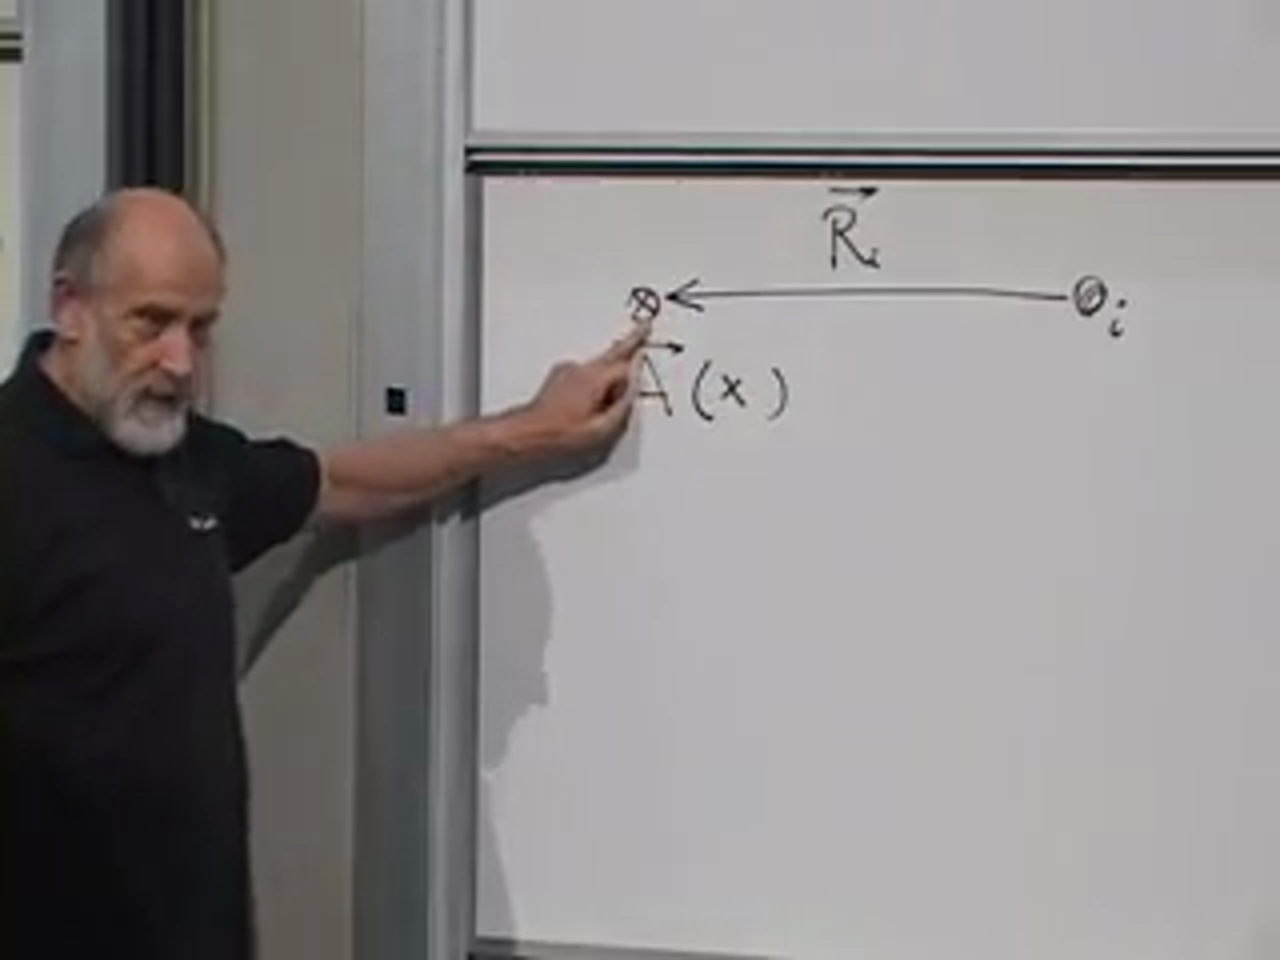
\includegraphics[width=0.82\textwidth]{lecture_02_figure_03.png}
  \caption{Source masses, a test point, and the displacement vector used to
  fix the direction of every term in the gravitational acceleration field.}
  \lectureframe{00:23:26}
\end{figure}

For a continuous distribution we replace a large collection of microscopic
sources by the mass density
\begin{equation}
  \rho(\vec x)
  =
  \lim_{\Delta V\to0}\frac{\Delta m}{\Delta V}.
  \label{eq:l02-density}
\end{equation}
The density is itself a scalar field. Newton's many-source equation can now
be summarized by a much more compact local statement.

\section{Gauss's Law and Gauss's Theorem}

The field equation for Newtonian gravity is
\begin{equation}
  \boxed{\boldsymbol{\nabla}\cdot\vec A=-4\pi G\rho.}
  \label{eq:l02-gauss-law}
\end{equation}
Positive mass makes the field point inward. What would be positive outward
divergence for a source is therefore negative here: an inward convergence.
Equation~\eqref{eq:l02-gauss-law} is \emph{Gauss's law for gravity}. It is a
physical law, equivalent to Newton's relation between mass and gravitational
acceleration.

\begin{figure}[tbp]
  \centering
  
\includegraphics[width=0.86\textwidth]{lecture_02_figure_04.png}
  \caption{The many-source acceleration field and its compact local
  replacement, \(\boldsymbol{\nabla}\cdot\vec A=-4\pi G\rho\).}
  \lectureframe{00:32:20}
\end{figure}

Gauss's \emph{theorem} is different. It is a mathematical identity valid
for any sufficiently regular vector field and any region \(V\) bounded by
the closed surface \(\partial V\):
\begin{equation}
  \boxed{
  \int_V
    \boldsymbol{\nabla}\cdot\vec A\,dV
  =
  \oint_{\partial V}
    \vec A\cdot\hat n\,d\sigma.}
  \label{eq:l02-divergence-theorem}
\end{equation}
The region need not be spherical. Subdivide its volume into tiny cells,
evaluate the divergence in each, multiply by the cell volume, and add.
Internal fluxes cancel between neighboring cells, leaving only the outward
normal component \(A_\perp=\vec A\cdot\hat n\) on the boundary.

\begin{figure}[tbp]
  \centering
  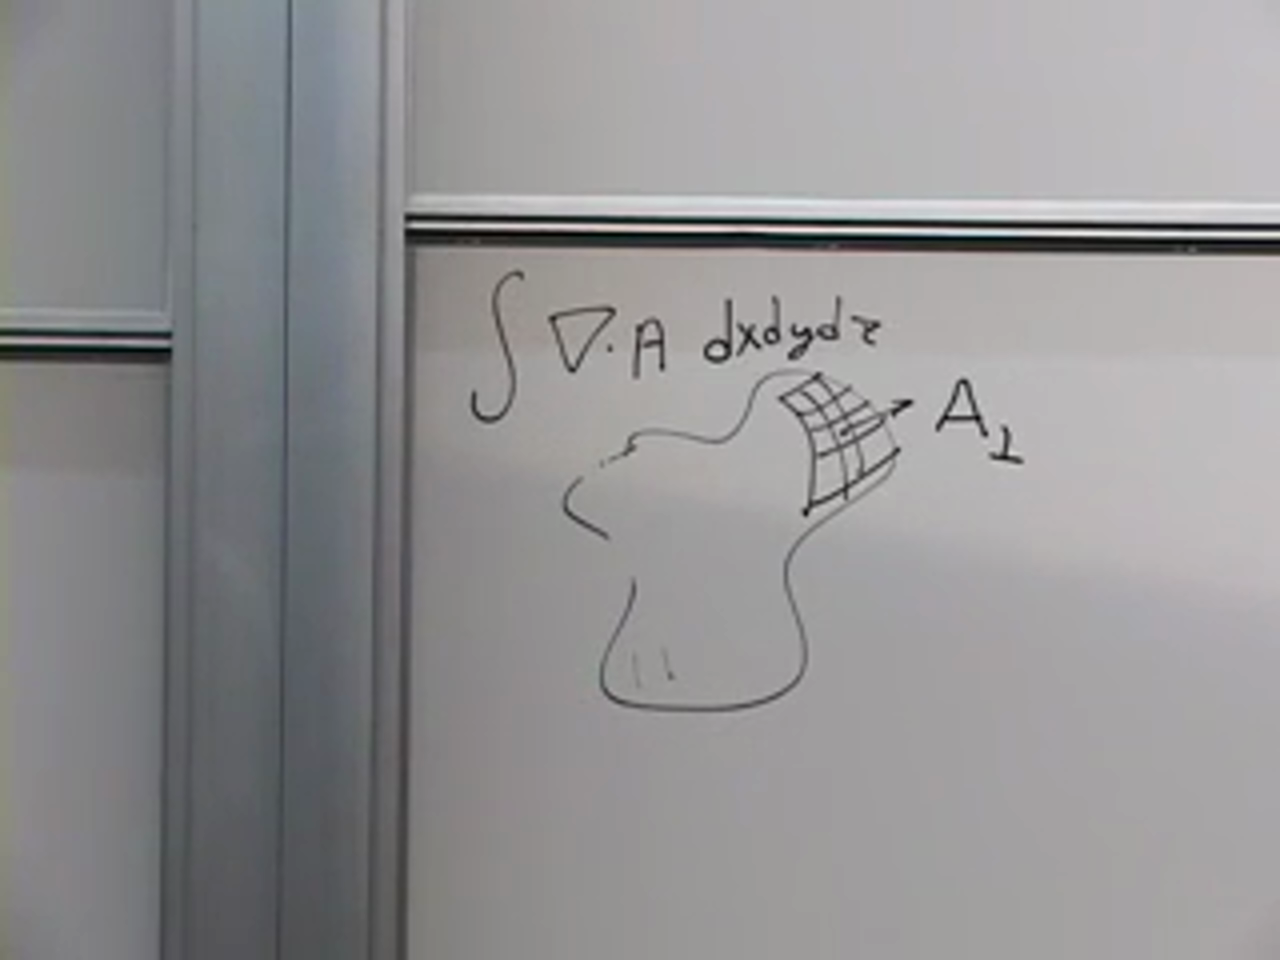
\includegraphics[width=0.82\textwidth]{lecture_02_figure_05.png}
  \caption{Gauss's theorem converts the integral of a volume divergence into
  the outward flux through the bounding surface. The marked surface patch
  carries area \(d\sigma\) and normal component \(A_\perp\).}
  \lectureframe{00:35:00}
\end{figure}

The fluid analogy makes the theorem immediate. If \(\vec A\) were a velocity
field, the integrated divergence would measure the net amount of fluid
created inside the region, and the surface integral would measure the amount
flowing out. Gauss's theorem equates these two descriptions. In gravity we
combine this mathematical theorem with the physical source law
\eqref{eq:l02-gauss-law}.

\section{Spherical Symmetry and the Exterior Field}

Take a spherically symmetric, or isotropic, mass distribution and surround
it with a concentric Gaussian sphere of radius \(r\). Integrating Gauss's
law gives
\begin{equation}
  \int_V
  \boldsymbol{\nabla}\cdot\vec A\,dV
  =
  -4\pi G\int_V\rho\,dV
  =
  -4\pi G M_{\mathrm{enc}}(r).
  \label{eq:l02-volume-side}
\end{equation}
Spherical symmetry forces the field to be radial and to have the same radial
component everywhere on the Gaussian sphere. If \(\hat r\) points outward,
\begin{equation}
  \oint_{\partial V}\vec A\cdot\hat n\,d\sigma
  =
  A_r(r)\,4\pi r^2.
  \label{eq:l02-surface-side}
\end{equation}
Equating the two sides,
\begin{equation}
  \begin{aligned}
    4\pi r^2 A_r
    &=
    -4\pi G M_{\mathrm{enc}}(r),\\
    &\boxed{
      A_r(r)
      =
      -\frac{G M_{\mathrm{enc}}(r)}{r^2}.}
  \end{aligned}
  \label{eq:l02-spherical-field}
\end{equation}
When the Gaussian sphere lies outside the whole body,
\(M_{\mathrm{enc}}=M\). Its exterior field is therefore exactly the field
of a point mass \(M\) at the center. This derivation also explains the
convenient \(4\pi\) in Gauss's law: it cancels the area \(4\pi r^2\) of a
sphere.

\begin{figure}[tbp]
  \centering
  
\includegraphics[width=0.88\textwidth]{lecture_02_figure_06.png}
  \caption{For an isotropic source, the volume integral gives the enclosed
  mass while the surface integral becomes \(4\pi r^2 A_r\), recovering the
  exterior inverse-square field.}
  \lectureframe{00:41:20}
\end{figure}

The compact divergence equation is equivalent to the cumbersome sum over
all source particles, but in a symmetric problem it does the calculation
almost at once.

\section{Inside a Uniform Earth}

The same method answers the question of the field inside the Earth. Choose a
Gaussian sphere of radius \(r<R\) within a model Earth of radius \(R\) and
uniform density \(\rho\). The real Earth is denser near its center, but
uniform density is sufficient to reveal the structure. The enclosed mass is
\begin{equation}
  M_{\mathrm{enc}}(r)
  =
  \frac{4\pi}{3}\rho r^3.
  \label{eq:l02-enclosed-uniform}
\end{equation}
Substitution into Equation~\eqref{eq:l02-spherical-field} gives
\begin{equation}
  \boxed{
  A_r(r)
  =
  -\frac{4\pi G\rho}{3}\,r,
  \qquad r<R.}
  \label{eq:l02-interior-field}
\end{equation}
At \(r=R\), this agrees with the exterior result because
\(M=(4\pi/3)\rho R^3\).

\begin{figure}[tbp]
  \centering
  
\includegraphics[width=0.86\textwidth]{lecture_02_figure_07.png}
  \caption{The inner Gaussian sphere and the rederived enclosed-mass
  calculation. Keeping the volume factor \(4\pi r^3/3\) and the \(4\pi\) in
  Gauss's law yields \(A_r=-(4\pi G\rho/3)r\).}
  \lectureframe{00:57:00}
\end{figure}

Multiplying the acceleration by a test mass \(m\) gives
\begin{equation}
  m\ddot r
  =
  -m\frac{4\pi G\rho}{3}r.
  \label{eq:l02-earth-oscillator}
\end{equation}
This is a harmonic oscillator with
\begin{equation}
  \omega^2=\frac{4\pi G\rho}{3}
  =\frac{GM}{R^3}
  =\frac{g_{\mathrm s}}{R},
  \label{eq:l02-earth-frequency}
\end{equation}
where \(g_{\mathrm s}=GM/R^2\) is the surface acceleration. A frictionless
tunnel through the idealized uniform Earth would therefore produce an
oscillation through the center and back.

The lecture makes an uncertain ten-minute estimate. Evaluating the model
instead gives
\begin{equation}
  T
  =
  \frac{2\pi}{\omega}
  =
  2\pi\sqrt{\frac{R}{g_{\mathrm s}}}
  \approx 84\ \mathrm{min}.
  \label{eq:l02-earth-period}
\end{equation}
The trip from one surface to the opposite surface is half a period, about
\(42\) minutes; the fall from the surface to the center is about
\(21\) minutes. The numerical correction leaves the point of the example
unchanged: Gauss's law solves a many-body problem which would be forbidding
as a direct sum.

\begin{classroomqa}
\audiencequestion{Why can the matter outside the Gaussian sphere be
neglected?
\lecturetimestamp{00:48:20--00:50:20}}
\lecturerresponse{It is not merely negligible; for spherical shells its net
field at every interior point is exactly zero. Contributions from the
different parts of an outer shell cancel. Thus only enclosed mass enters
\(A_r(r)\). A thin spherical shell has zero field inside and the same
exterior field as a point mass at its center. Newton established this
geometrically before the flux formulation made the cancellation immediate.}
\end{classroomqa}

\begin{classroomqa}
\audiencequestion{Is the gravitational field continuous across a shell?
\lecturetimestamp{00:53:02--00:53:40}}
\lecturerresponse{Across an ideal shell of zero thickness and finite surface
mass density, the normal component of the field jumps. A shell with finite
thickness replaces that jump by a smooth change through the material. The
ideal discontinuity is the limiting form of Gauss's law.}
\end{classroomqa}

\begin{classroomqa}
\audiencequestion{If enclosed mass grows as \(r^3\), why does the interior
field grow only linearly with \(r\)?
\lecturetimestamp{00:53:40--00:57:12}}
\lecturerresponse{The flux also contains the Gaussian-sphere area,
proportional to \(r^2\). Hence
\[
  A_r r^2\propto M_{\mathrm{enc}}\propto r^3
  \quad\Longrightarrow\quad
  A_r\propto r.
\]
The spoken conclusion \(1/r\) during the live algebra is a slip; the
rederivation immediately returns to the correct linear field. The
coefficient is fixed by retaining every \(4\pi\):
\(A_r=-(4\pi G\rho/3)r\).}
\end{classroomqa}

Gravitational potential is announced at this point but deliberately
postponed. We move instead from this old physics to the equivalence
principle.

\section{The Accelerating Elevator}

Let an elevator accelerate horizontally with magnitude \(g\). A released
object can remain at rest in an inertial frame outside while the elevator
moves beneath it. The passenger describes the same event differently: the
object accelerates toward the floor with acceleration \(-g\). Every freely
released body behaves in the same way, just as it would in a uniform
gravitational field.

\begin{figure}[tbp]
  \centering
  
\includegraphics[width=0.72\textwidth]{lecture_02_figure_08.png}
  \caption{The horizontal elevator accelerates to the right. In the
  passenger's frame a released object accelerates toward the rear floor,
  producing the appearance of a uniform gravitational field.}
  \lectureframe{01:01:20}
\end{figure}

The observation sounds elementary. Einstein's step was to use it as a
principle applying not merely to dropped masses but to all local physics.
Before doing that, let us express the change of frame mathematically.

\subsection{Uniform Velocity}

Place \(x\) horizontally and \(t\) vertically on a spacetime diagram.
Suppose first that the elevator moves with constant velocity \(v\), and call
its floor \(x'=0\). Newtonian coordinates are related by the Galilean
transformation
\begin{equation}
  x'=x-vt,
  \qquad
  t'=t.
  \label{eq:l02-galilean}
\end{equation}
The equality \(t'=t\) belongs to Newtonian physics and will be modified in
special relativity.

If a ball is at rest outside, then \(x\) is constant, and
\begin{equation}
  \dot x'=-v,
  \qquad
  \ddot x'=0.
  \label{eq:l02-uniform-derivatives}
\end{equation}
The moving passenger sees the ball pass backward, but sees no acceleration.
Uniform relative motion creates no gravitational field.

\begin{figure}[tbp]
  \centering
  
\includegraphics[width=0.82\textwidth]{lecture_02_figure_09.png}
  \caption{Straight worldlines for the stationary and uniformly moving
  coordinate grids, together with the Galilean transformation
  \(x'=x-vt,\ t'=t\).}
  \lectureframe{01:10:20}
\end{figure}

\subsection{Uniform Acceleration}

Now let the elevator start from rest and accelerate uniformly. Its floor
follows
\begin{equation}
  x_{\mathrm{floor}}(t)=\frac12 gt^2,
  \label{eq:l02-floor}
\end{equation}
a parabola in the \(x\)-\(t\) diagram. Coordinates carried by the elevator
are therefore
\begin{equation}
  x'=x-\frac12 gt^2.
  \label{eq:l02-accelerated-transform}
\end{equation}
For a ball at rest in the outside inertial frame,
\begin{equation}
  \dot x'=-gt,
  \qquad
  \boxed{\ddot x'=-g.}
  \label{eq:l02-effective-gravity}
\end{equation}
This is the elevator argument in equations. An accelerated frame is a
curvilinear coordinate system in spacetime, and in those coordinates a
force-free body acquires the apparent acceleration of a uniform
gravitational field.

\begin{figure}[tbp]
  \centering
  
\includegraphics[width=0.86\textwidth]{lecture_02_figure_10.png}
  \caption{The accelerated coordinate transformation and its two time
  derivatives. Curved coordinate worldlines yield the effective
  acceleration \(\ddot x'=-g\).}
  \lectureframe{01:16:20}
\end{figure}

This is the first bridge between gravity and curvature: acceleration is
represented by curved coordinate lines. It is not yet spacetime curvature,
because the underlying Newtonian spacetime has not changed. The distinction
between curved coordinates and genuinely curved geometry will matter at the
end of the lecture.

\section{Light Falls}

The equivalence principle is powerful only if it applies to every local law
of physics. Consider an elevator accelerating upward. A horizontal beam is
emitted at the instant the elevator begins to accelerate. In the outside
inertial frame the light travels straight while the cabin rises. In the
elevator frame the beam therefore strikes the far wall below its original
height and traces a downward parabola. Its transverse acceleration is
\(-g\).

\begin{figure}[tbp]
  \centering
  
\includegraphics[width=0.72\textwidth]{lecture_02_figure_11.png}
  \caption{A horizontal light beam in an upward-accelerating elevator. The
  rising cabin makes the beam's path curve downward in the passenger's
  coordinates, showing that light falls in a gravitational field.}
  \lectureframe{01:20:20}
\end{figure}

\begin{classroomqa}
\audiencequestion{What happens if the light is sent along the direction of
the elevator's acceleration?
\lecturetimestamp{01:20:36--01:21:01}}
\lecturerresponse{The effect is then longitudinal rather than a transverse
bending. It changes the light's energy, and therefore its frequency, rather
than changing the locally measured speed \(c\). This is the seed of the
gravitational frequency-shift argument.}
\end{classroomqa}

\subsection{A Crude Solar-Deflection Estimate}

Take a ray that just skims the Sun, whose mass and radius are \(M\) and
\(R\). Near closest approach, approximate the downward acceleration by the
surface value
\begin{equation}
  g_\odot\approx\frac{GM}{R^2}.
  \label{eq:l02-solar-g}
\end{equation}
The ray spends roughly one solar diameter in the strong-field region, so
\begin{equation}
  \Delta t\approx\frac{2R}{c}.
  \label{eq:l02-crossing-time}
\end{equation}
Its acquired transverse velocity is then
\begin{equation}
  \Delta v_\perp
  \approx
  g_\odot\Delta t
  \approx
  \frac{2GM}{Rc}.
  \label{eq:l02-transverse-velocity}
\end{equation}
For a small angle,
\begin{equation}
  \boxed{
  \theta_{\mathrm{Newton}}
  \approx
  \frac{\Delta v_\perp}{c}
  \approx
  \frac{2GM}{Rc^2}.}
  \label{eq:l02-newton-deflection}
\end{equation}

\begin{figure}[tbp]
  \centering
  
\includegraphics[width=0.88\textwidth]{lecture_02_figure_12.png}
  \caption{The sun-skimming ray estimate combines
  \(g_\odot\approx GM/R^2\) with a crossing time \(2R/c\) to obtain the
  weak-field deflection scale \(2GM/(Rc^2)\).}
  \lectureframe{01:27:20}
\end{figure}

\begin{classroomqa}
\audiencequestion{Would ordinary Newtonian mechanics, applied to a photon
with effective mass \(E/c^2\), predict the observed bending?
\lecturetimestamp{01:21:03--01:28:22}}
\lecturerresponse{It gives the estimate
\(2GM/(Rc^2)\), the same result obtained from this elementary equivalence
argument. The full general-relativistic result is not half of this value but
exactly twice it:
\[
  \theta_{\mathrm{GR}}=\frac{4GM}{Rc^2}.
\]
The extra factor reflects spatial curvature, which the Newtonian estimate
does not include. The solar deflection was tested by comparing stellar
positions near the Sun during an eclipse.}
\end{classroomqa}

The historical point is larger than the rough numerical calculation.
Gravity and acceleration had long been compared mechanically; Einstein
applied the equivalence to light and electromagnetic phenomena, where its
consequences were new.

\section{Why Equivalence Is Local}

A single uniformly accelerated frame cannot reproduce the whole field of a
round Earth. The gravitational acceleration points in different directions
at different places and changes in magnitude with radius. It can be made
uniform only within a region too small, and during a time too short, to
resolve those variations.

\begin{figure}[tbp]
  \centering
  
\includegraphics[width=0.74\textwidth]{lecture_02_figure_13.png}
  \caption{The Earth's radial field cannot be replaced globally by one
  uniformly accelerating elevator. Its changing direction and magnitude
  leave measurable relative accelerations.}
  \lectureframe{01:31:20}
\end{figure}

A freely falling observer small enough to sample only one point can remove
gravity locally. An extended observer cannot. The feet, being nearer the
Earth, accelerate more strongly than the head; neighboring vertical
trajectories spread or contract because their directions differ. The body
is stretched radially and squeezed transversely. These relative
accelerations are tidal forces.

Tidal forces are the invariant remainder of gravity in this argument. A
uniform field has zero spatial variation and can be canceled by uniform
acceleration. A realistic field has nonzero spatial derivatives; where mass
is present, its divergence obeys
\(\boldsymbol{\nabla}\cdot\vec A=-4\pi G\rho\), while tidal derivatives can
remain nonzero even in the surrounding vacuum. No single accelerated
coordinate system can remove those variations over an extended region.

\begin{classroomqa}
\audiencequestion{Does special relativity still hold inside the local
elevator?
\lecturetimestamp{01:36:18--01:36:35}}
\lecturerresponse{Yes. In a sufficiently small freely falling laboratory,
local physics is special relativistic and inertial frames are related by
Lorentz transformations. The coordinate calculations above used the
Newtonian approximation only to establish the elementary elevator picture;
the relativistic refinement is deferred.}
\end{classroomqa}

\section{The Metric and the Meaning of Curvature}

We finish by isolating the geometric language needed later. A geometry is
determined by the distances between neighboring points. In rectangular
Cartesian coordinates on a flat blackboard, Pythagoras gives
\begin{equation}
  ds^2=dx^2+dy^2.
  \label{eq:l02-euclidean-metric}
\end{equation}
The same flat board may be covered by curved coordinate lines. In general
coordinates its infinitesimal distance takes the quadratic form
\begin{equation}
  \boxed{
  \begin{aligned}
    ds^2
    &=
    g_{xx}(x,y)\,dx^2
    +2g_{xy}(x,y)\,dx\,dy\\
    &\quad
    +g_{yy}(x,y)\,dy^2.
  \end{aligned}}
  \label{eq:l02-general-metric}
\end{equation}
The three coefficient functions form the two-dimensional metric. The
off-diagonal coefficient \(g_{xy}\) records the failure of the coordinate
directions to be perpendicular. The diagonal coefficients record the local
scale of coordinate intervals; if the grid stretches or compresses from
place to place, they depend on position.

\begin{figure}[tbp]
  \centering
  
\includegraphics[width=0.88\textwidth]{lecture_02_figure_14.png}
  \caption{Cartesian and curvilinear coordinate meshes with their metric
  forms. A complicated metric can describe a flat board merely because the
  coordinates are complicated.}
  \lectureframe{01:42:20}
\end{figure}

Curved coordinate lines do not by themselves imply curved geometry. A
geometry is flat if some coordinate choice reduces its metric to the
Euclidean form \eqref{eq:l02-euclidean-metric} throughout the region under
consideration. If no coordinate transformation can do so, the geometry is
intrinsically curved.

The examples make the distinction concrete:
\begin{itemize}
  \item A plane is flat.
  \item A sphere is curved; no coordinate grid makes its metric globally
        Pythagorean.
  \item A cylinder is intrinsically flat because it can be cut and unrolled
        onto a plane without stretching.
  \item A saddle is curved.
  \item A cone is flat away from its tip; its curvature is concentrated at
        the singular tip.
\end{itemize}

Curvature is the obstruction to flattening a metric by a change of
coordinates. Tidal acceleration is the obstruction to eliminating gravity
by a change to a freely falling frame. These are not merely analogous
statements. General relativity will identify spacetime curvature with the
tidal content of the gravitational field.

\section{What We Have Established}

The argument has moved through three layers. Newtonian gravity first became
a field theory:
\begin{equation}
  \vec A(\vec x)
  =
  G\sum_i m_i\frac{\vec R_i}{R_i^3},
  \qquad
  \boldsymbol{\nabla}\cdot\vec A=-4\pi G\rho.
\end{equation}
Gauss's theorem then turned that local source equation into the exterior
inverse-square field, the shell theorem, and the linear interior field of a
uniform Earth.

Next, an accelerated coordinate system produced an apparent uniform field,
\(\ddot x'=-g\). Applying that equivalence to all local physics showed that
light falls and supplied the correct scale, though not yet the full factor,
for solar light deflection.

Finally, the limitation of the elevator became the opening to geometry.
Uniform gravity can be removed locally; tidal forces cannot. Curved
coordinates can describe a flat surface; intrinsic curvature cannot be
removed. The next task is to make that connection between tidal gravity and
spacetime curvature precise.
